\begin{figure}[!t]
\centering
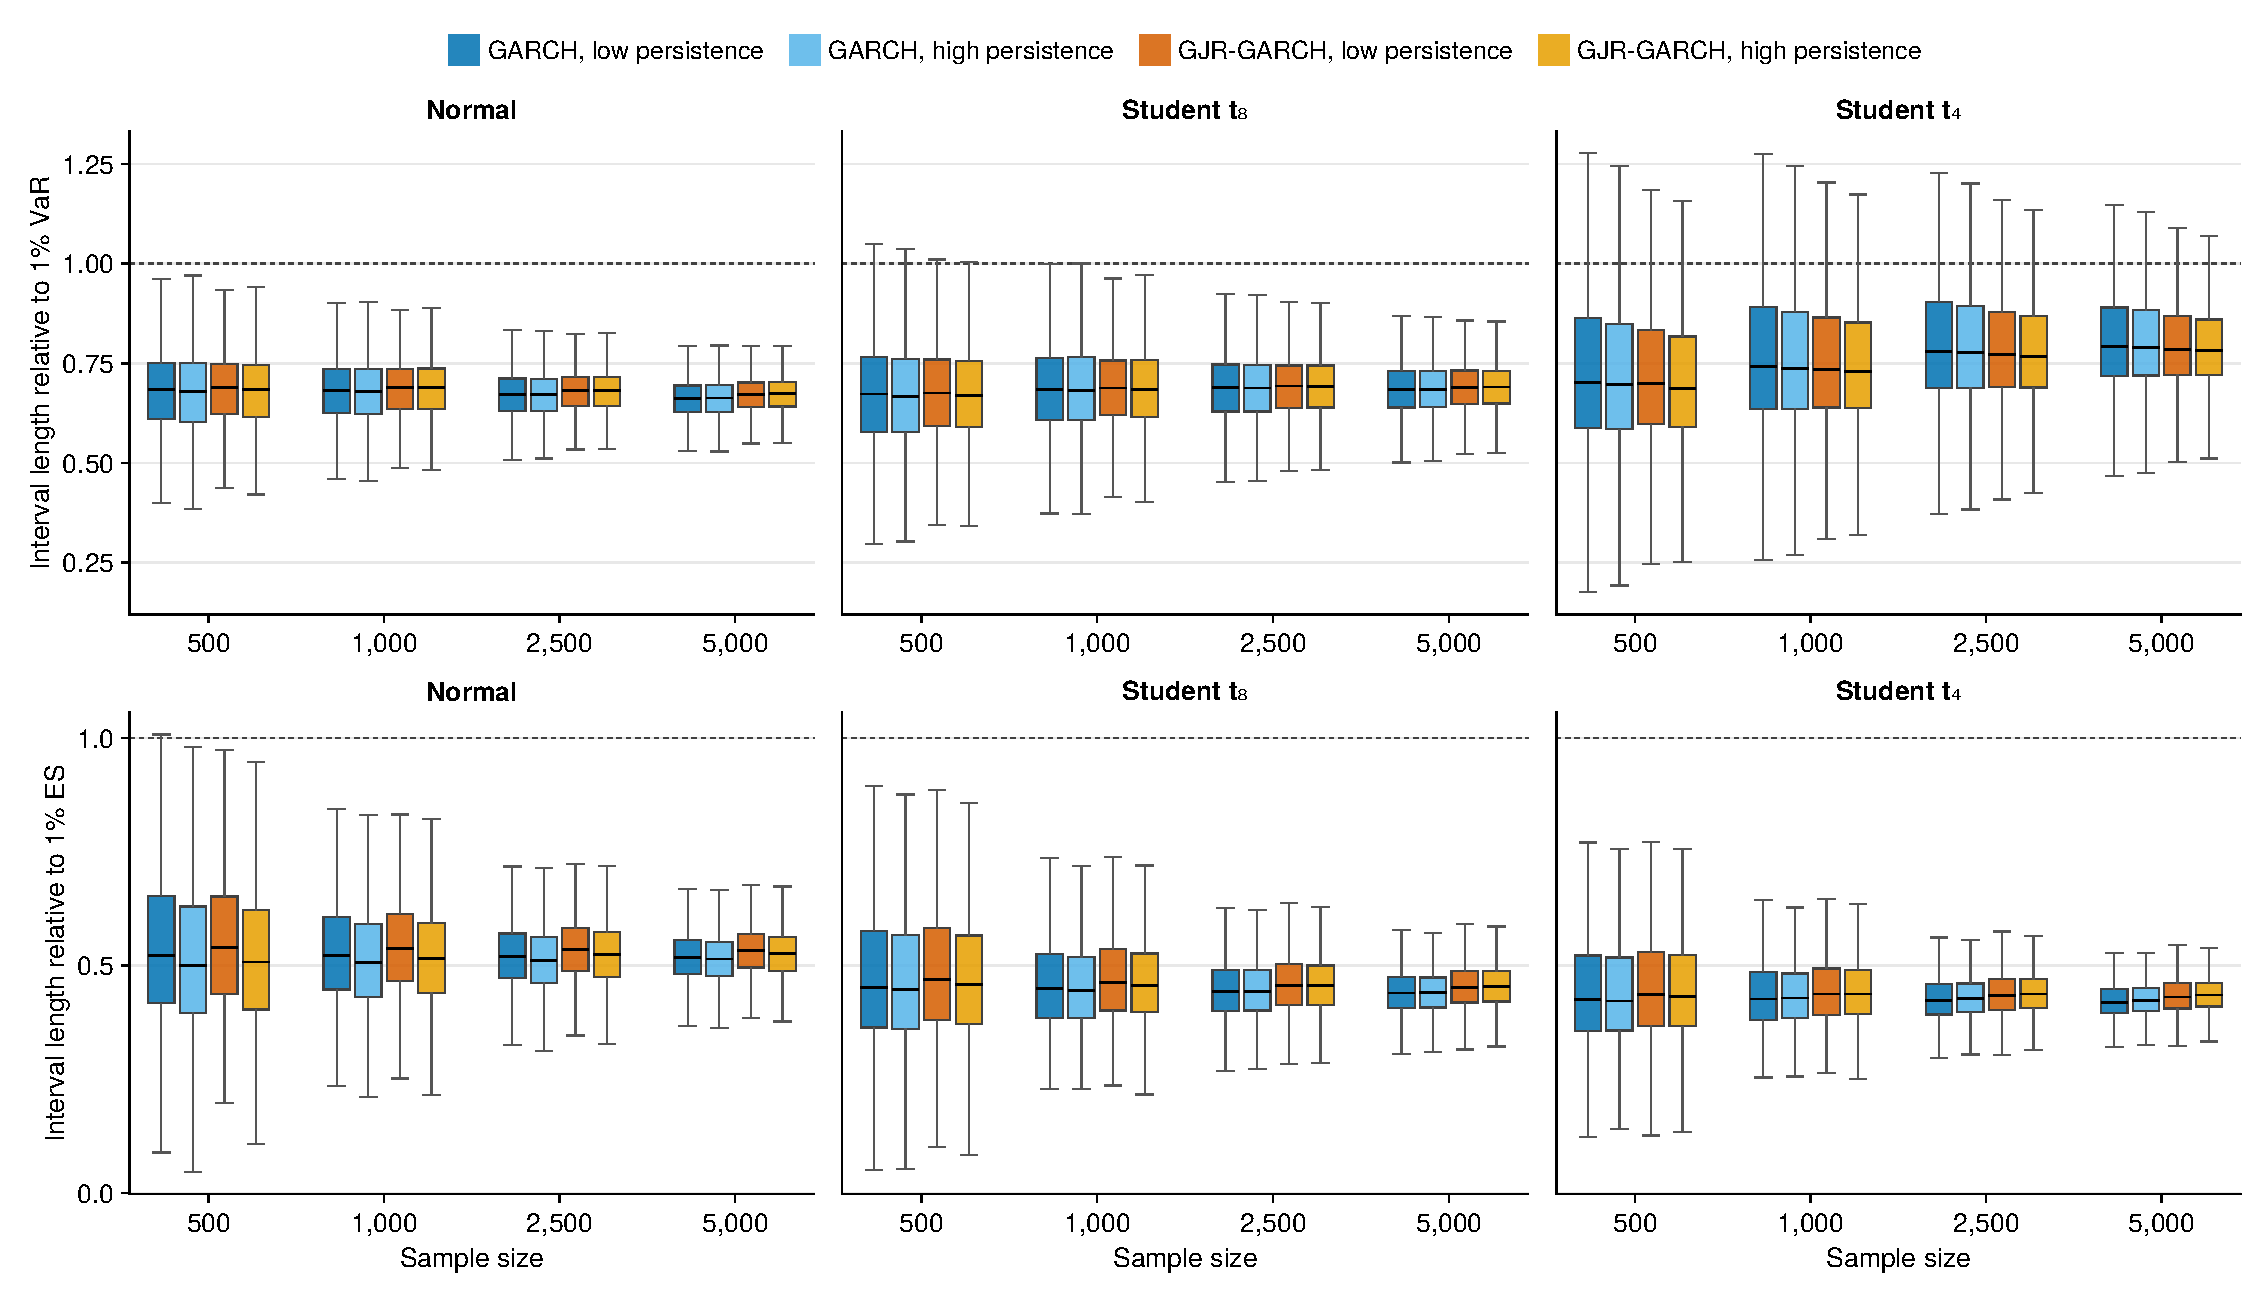
\includegraphics[width=\textwidth]{../results/mc/figures/mc_interval_length_ratios_0p01.pdf}
\caption{Relative lengths of confidence intervals for conditional risk measures at 1\%. Each box summarizes the replication-level ratio between the length of the nominal 95\% Wald interval for the conditional expectile at $\tau=0.01$ and the corresponding interval length for VaR at $\alpha=0.01$ (top row) or ES at $\delta=0.01$ (bottom row). Thus, $\alpha=\delta=\tau$. The dashed reference line at one denotes equal interval lengths; values below one indicate a shorter expectile interval. Boxes show the interquartile range and median, whiskers extend to 1.5 times the interquartile range, and more extreme observations are omitted from the display. The calculations retain every finite, positive interval-length ratio in the raw Monte Carlo CSV.}
\label{fig:mc-interval-length-ratios-0p01}
\end{figure}
